% !TEX encoding = UTF-8
% !TEX program = pdflatex
% !TeX spellcheck = en_GB
% !BIB = biber

\documentclass[english]{article}
\usepackage{amsmath}
\usepackage{wasysym}
\usepackage{amssymb}
\usepackage{babel}
\usepackage[utf8]{inputenc}
\usepackage{graphicx}
\usepackage[obeyspaces]{url}
\graphicspath{{./images/}}
\usepackage{hyperref}
\hypersetup{
    colorlinks=true, 
	linkcolor=blue, 
	filecolor=blue, 
	citecolor = black,       
	urlcolor=blue, 
}
\usepackage{listings}
\lstset{
  xleftmargin=15pt,
  xrightmargin=0pt,
  framexleftmargin=0pt,
  framexrightmargin=0pt,
  basicstyle={\fontsize{9pt}{10pt}\ttfamily},
  columns=flexible,
  numbers=left,
  numbersep=10pt,
  numberstyle={\fontsize{9pt}{11pt}\selectfont\color[rgb]{0.4,0.4,0.1}},
  keepspaces=true,
  showstringspaces=false,
  identifierstyle=\color[rgb]{0.1,0.1,0.1},
  keywordstyle=\color{blue},
  commentstyle=\color[rgb]{0,0.3,0},
  morekeywords={rule, lemma},
  morekeywords=[2]{let, in},
  morekeywords=[3]{Fr, pk},
  morekeywords=[4]{In, Out},
  morekeywords=[5]{senc, aenc, h}
  morecomment=[s][keywordstyle3]{/*}{/},
  keywordstyle=\color[rgb]{0.44,0.57,0.65},
  stringstyle=\color{green},
  keywordstyle=[2]{\color[rgb]{0.86,0.57,0.18}},
  keywordstyle=[3]{\bfseries\color[rgb]{0,0.3,0.2}}
  }
\usepackage{biblatex}
\addbibresource{thud.bib}

\title{A Temporal Logic Based Framework for Intrusion Detection}
\author{Zanolin Lorenzo}

\begin{document}

\maketitle

\begin{abstract}
The purpose of this paper is to introduce MONID, which is a framework created for system intrusion detection. This framework uses EAGLE, a rich and effectively monitorable logic, to express intrusion patterns using temporal logic formulas; EAGLE's ability to include data values and parameterized recursive equations makes it possible to represent security threats that include complex temporal event sequences and attacks with intrinsically statistical signatures succinctly. This tool can be used in offline and real-time scenarios. The implementation uses an algorithm for online monitoring that matches descriptions of the lack of an assault with indications of system execution; an alarm is set off whenever the standard is broken.
\end{abstract}

\tableofcontents
\newpage

\section{Introduction}
Even with all of the advances in computer security research, totally safe computer systems remain a long way off. Almost every large and complicated computer system nowadays contains vulnerabilities. Intrusion detection means maintaining constant surveillance on a system in order to detect any misuse of these weak areas as soon as feasible so that they can be repaired.

There are three Intrusion Detection System approaches, according to the literature: \textit{signature-based}\cite{gao2014cyber}, \textit{anomaly-based}\cite{jyothsna2011review} and \textit{hybrid}\cite{garg2016hybrid}. The first approach aims to identify patterns and match them with known signs of intrusions relying on a database of previous intrusions. If activity within the network matches the “signature” of an attack or breach from the database, the detection system creates an alert. This approach has a low false-alarm rate, but it requires us to know the patterns of security attacks in advance and previously unknown attacks would go undetected. In contrast, \textit{anomaly-based} is capable to detect new attacks since an alarm is raised if an observed behavior deviates significantly from pre-learned normal behavior. Finally, a \textit{hybrid system} combines the best of both worlds by looking at patterns and one-off events, a Hybrid Intrusion Detection system can flag new and existing intrusion strategies. 

In this paper we will focus on \textit{signature-based} approach using temporal logic; we use EAGLE\cite{barringer2004rule,barringer2003eagle} to specify a system's attack-safe behavior. EAGLE allows recursively built temporal formulas, parameterizable by both logical formulas and data expressions, across three primitive modalities: "next", "previous", and "concatenation". The logic allows us to describe temporal patterns involving reasoning about data-values observed in individual events. Unlike LTL, EAGLE allows us to design attacks with fundamentally statistical characteristics; password guessing attacks and ICMP-flood denial of service attacks are two examples. We will monitor EAGLE formulas using an online algorithm that processes each event as it happens and updates the monitored formula to store a relevant summary. An intrusion alarm is triggered if, for any reason, the updated formula turns out to be false; as a result, the entire process operates in real-time. We'll see how the implementation, MONID, examines the event stream to see if the monitored formula (which is used to hold the pertinent summary of the system) is being broken.

%% INTRODURRE VELOCE ESEMPIO E STRUTTURA DEL PROGRAMMA
%%%%%   DA RISCRIVERE ALLA FINE
In Section 2, we'll deeply explore EAGLE, covering everything from its syntax to semantics and the evaluation algorithm, with the add of practical examples. Moving on to Section 3, we'll delve into the MONID framework, which employs EAGLE to construct an intrusion detection system. Section 4 will focus on specific EAGLE rules tailored for the detection of various types of attacks and finally, in Section 5, we will draw our conclusions.
%%%%5

\section{EAGLE, a Temporal Monitoring Logic}
According to~\cite{barringer2004program}, EAGLE offers a succinct but powerful set of primitives, supporting recursive parameterized equations with a minimal/maximal fix-point semantics together with three temporal operators: next-time ($\bigcirc$), previous-time ($\astrosun$), and concatenation ($\cdot$).
\subsection{Basics}\label{sec:ltl}
In EAGLE recursion definitions are supported; as exmaple, in the current framework we can build the following definitions:
\begin{align*}
& \underline{\text{min}}\ \mathtt{Next}(\underline{\text{Form}}\ F) = \bigcirc F \\
& \underline{\text{max}}\ \mathtt{Always}(\underline{\text{Form}}\ F) = F \land \bigcirc \mathtt{Always}(F) \\
& \underline{\text{min}}\ \mathtt{Eventually}(\underline{\text{Form}}\ F) = F \lor \bigcirc \mathtt{Eventually}(F) \\
& \underline{\text{min}}\ \mathtt{Until}(\underline{\text{Form}}\ F_1, \underline{\text{Form}}\ F_2) = F_2 \lor (F_1 \land \bigcirc \mathtt{Until}(F_1,F_2))
\end{align*}

As we can see, rules are parameterized by an EAGLE formula (of type $\underline{\text{Form}}$), which means that we will be able to write EAGLE formulas such as $\mathtt{Always}(\mathtt{Eventually}(x>0))$. Also, the $\mathtt{Always}$ operator is defined as maximal solution of the equation $X=F\land \bigcirc X$, while the $\mathtt{Eventually}$ operator represents the minimal solution to the equation $X=F\lor \bigcirc X$.

Assume that we want to state the following property: "\textit{Whenever there is a login by any user x, then eventually the user x logs out}". In LTL we can write the following formula: 
\begin{align*}
    & \square{((action = \mathtt{login})\rightarrow \underline{\text{let}}\ k=userId\ \underline{\text{in}}\ \lozenge(action = \mathtt{logout}\land userId = k))}
\end{align*}
In this formula we use the operator \underline{let} \_ \underline{in} \_ to bind the value of $userId$ in the current event to the local variable $k$ whenever $(action = \mathtt{login})$ in the current event; we then impose the condition that the value of $userId$ in some event in future must be same as the user id bound to k and that the action of the event must be logout.
In EAGLE we can express the same property with the following rules:
\begin{align*}
    & \underline{\text{min}}\ \mathtt{EvLogout}(\underline{\text{string}}\ k) = (action = \mathtt{logout}\land userId = k) \lor \bigcirc \mathtt{EvLogout}(k) \\
    & \underline{\text{mon}}\ M_2 = ((action = \mathtt{login})\rightarrow \mathtt{EvLogout}(userId)) 
\end{align*}
As a result, rules in EAGLE give us the power to create specific temporal operators as well as to bind and modify data. This property turns out to be crucial for succinctly expressing executions of attack-safe systems. As we can see, each rule begins with a term that describes its type ($\underline{\text{min}}$, $\underline{\text{max}}$, $\underline{\text{mon}}$); we will read more about it later.

Lastly, two assumptions must be made:\begin{enumerate}
    \item There is a finite sequence of events called $\sigma=\alpha_{1},\ldots ,\alpha_{n}$ that is a merge of the system registered logs organized by ascending time. 
    The structure of an event record $\alpha_i$ is the following:
    \begin{align*}
        & \mathtt{LoginLogoutEvent}\{userId:\underline{\text{string}},\ action: \underline{\text{int}},\ time: \underline{\text{double}}\} 
    \end{align*}
    An example of event could be: $\{userId:\mathtt{"Lori"},\ action:\mathtt{login},\ time:\mathtt{20}\}$
    \item For each attack, there is a formula $F$ which specifies the absence of it.
\end{enumerate}
To make the paper self-contained, we will present the syntax and semantics of EAGLE.

\subsection{Syntax and Semantics}
\textbf{Syntax.}
A specification $S$ is made up of an observer part $O$ and a declaration part $D$. $O$ is made up of zero or more monitor definitions $M$, which define what will be watched, while $D$ is made up of zero or more rule definitions $R$. The names of rules and monitors are $(N)$.
\begin{align*}
    S &::= D \, O \\
    D &::= R^* \\
    O &::= M^* \\
    R &::= \{\underline{\text{max}}\ |\ \underline{\text{min}} \}\ N(T_1\ x_1, \ldots, T_n\ x_n) = F \\
    M &::= \underline{\text{mon}}\ N = F \\
    T &::= \underline{\text{Form}}\ |\ \text{primitive type} \\
    F &::= \text{expression}\ |\ \underline{\text{true}}\ |\ \underline{\text{false}}\ |\ \neg F\ |\ F_1 \land F_2\ |\ F_1 \lor F_2\ |\\
            &F_1 \rightarrow F_2\ |\ \bigcirc F\ |\ \odot F\ |\ F_1 \cdot F_2\ |\ N(F_1, \ldots, F_n)\ |\ x_i
\end{align*}
The types $T_i$ of parameters include primitive types like \underline{int}, \underline{long}, \underline{float}, etc. or formulas of type \underline{Form}. Definitions starting with keyword $\underline{\text{mon}}$ specifies the EAGLE formulas to be monitored and cannot have a recursive definition. We will see that these kind of rules will evolve as new events appear. 
A term indicating whether the interpretation is maximal ($\underline{\text{max}}$) or minimal ($\underline{\text{min}}$) comes before a rule specification $R$. While minimal rules establish \textit{liveness properties} (something good eventually happens), maximal rules define \textit{safety properties} (nothing bad ever happens); we shall see that the difference becomes important only when we are evaluating the at the boundaries of a trace. Finally, recursive definitions of rules are permitted as long as they are tightly guarded by a temporal operator. 

\textbf{Semantics.} The semantics of the logic is defined in terms of the \textit{satisfaction} relation $\models$ which defines whether a finite execution trace $\sigma$ satisfies the specification $\varphi=D \, O$. The $i$'th state $s_i$ of a trace $\sigma$ is denoted by $\sigma(i)$. The term $\sigma[i, j]$ denotes the sub-trace of $\sigma$ from position $i$ to position $j$, both positions included; if $i \geq j$ then $\sigma[i, j]$ denotes the empty trace.

Given a trace $\sigma$ and a specification $D \, O$, satisfaction is defined as follows:
\[
\sigma \models D \, O \text{ iff } \forall (\underline{\text{mon}}\ N = F) \in O.\ \sigma ,1 \models_D \, F
\]
In other words, a trace satisfies a specification if it fulfills each monitored formula ($\underline{\text{mon}}$) when monitoring from position 1, which is the initial state. The definition of the satisfaction relation $\models_D \subseteq (Trace \times \mathbb{N}) \times \underline{\text{Form}}$, for a set of rule definitions $D$, is the following:
\begin{align*}
    \sigma, i &\models_D\ expression &\text{iff} \quad &1 \leq i \leq |\sigma|\ \text{and}\ evaluate(expression, \sigma(i)) = true \\
    \sigma, i &\models_D\ \underline{\text{true}} \\
    \sigma, i &\not\models_D\ \underline{\text{false}} \\
    \sigma, i &\models_D \neg F &\text{iff} \quad &\sigma, i \not\models_D F \\
    \sigma, i &\models_D F_1 \land F_2 &\text{iff} \quad &\sigma, i \models_D F_1\ \text{and}\ \sigma, i \models_D F_2 \\
    \sigma, i &\models_D F_1 \lor F_2 &\text{iff} \quad &\sigma, i \models_D F_1\ \text{or}\ \sigma, i \models_D F_2 \\
    \sigma, i &\models_D F_1 \rightarrow F_2 &\text{iff} \quad &\sigma, i \models_D F_1 \text{ implies } \sigma, i \models_D F_2 \\
    \sigma, i &\models_D \bigcirc F &\text{iff} \quad &i \leq |\sigma|\ \text{and}\ \sigma, i+1 \models_D F \\
    \sigma, i &\models_D \odot F &\text{iff} \quad &1 \leq i\ \text{and}\ \sigma, i-1 \models_D F \\
    \sigma, i &\models_D F_1 \cdot F_2 &\text{iff} \quad &\exists j \text{ s.t. } i \leq j \leq |\sigma|+1\ \text{and}\ \sigma^{[1, j-1]}, i \models_D F_1\ \text{and}\ \sigma^{[j,|\sigma|]}, 1 \models_D F_2 \\
    \sigma, i &\models_D N(\overline{F}, \overline{P}) &\text{iff} 
    &\begin{cases}
    \text{if } 1 \leq i \leq |\sigma| \text{ then:} \\
    \quad \sigma, i \models_D F[ \overline{f} \mapsto \overline{F}, \overline{p} \mapsto\ evaluate(\overline{P}, \sigma(i))] \\
    \quad \text{where } (N(\underline{\overline{\text{Form}}}\ \overline{f}, \text{T } p) = F) \in D \\
    \text{otherwise, if } i = 0 \text{ or } i = |\sigma|+1 \text{ then:} \\
    \quad \text{rule } N \text{ is defined as }\underline{\text{max}}\text{ in } D
    \end{cases}
\end{align*}
where $\overline{F}$ and $\overline{P}$ represent tuples of type $\overline{\text{Form}}$ and $\overline{T}$ respectively
    
An \textbf{important} note is that, given a trace $\sigma=\alpha_{1},\ldots ,\alpha_{n}$ the index $i$ of the trace can become $0$ (before the first state) and $n+1$, thus going beyond the limits; both of these situations result in rule applications evaluating to either true if maximal or false if minimal, without first taking the rules body into account. Let us explain why using an example. Given the definition 
\begin{align*}
    & \underline{\text{min}}\ \mathtt{Property}(\underline{\text{Form}}\ F) =F \lor \bigcirc \mathtt{Property}(F)
\end{align*}
and the sequence $\sigma=\alpha_{1},\ldots ,\alpha_{n}$, Property will evaluate to \textit{true} 
\begin{align*}
    & evaluate(\ldots evaluate(evaluate(\mathtt{Property},\alpha_1),\alpha_2),\ldots,\alpha_n)=true
\end{align*}
if and only if the rule is true at some given event $\alpha_i$. 
Once the sequence has been completely analyzed, we will obtain a big disjunction (in case of a \underline{\text{min}}) or a big conjunction (in case of a \underline{\text{max}}) and the final value will close the evalutation. Continuing the example, the extended formula will be:
\begin{align*}
    & F \lor \bigcirc(F \lor \bigcirc(\ldots F \lor \bigcirc \mathbf{Property(F)})) 
\end{align*}
and the bold $\mathbf{Property(F)}$ will be evaluated to false, since it is the last of a big disjunction.
\subsection{Evaluation algorithm}\label{algo}
As already mentioned, monitored formulas ($\underline{\text{mon}}$) evolve at every event, to store relevant informations about past istants. The evolved formula's value is determined at the conclusion of the event series; if it is true, the formula is satisfied by the event sequence; otherwise, it is violated. Formally, a formula $F' = evaluate(F, \alpha_i)$ is created when a formula $F$ is evaluated at an event $\alpha_i = \sigma(i)$ and has the condition that $\sigma, i \models F$ if and only if $\sigma, i+1 \models F'$. With $F$ being the evolved formula, we compute the boolean function $value(F)$ at the conclusion of the trace. The definition of the function $evaluate: \underline{\text{Form}} \times \underline{\text{State}} \to \underline{\text{Form}}$ uses an auxiliary function $update: \underline{\text{Form}} \times \underline{\text{State}} \to \underline{\text{Form}}$ to pre-evaluate a formula if it is guarded by the previous operator $\bigodot$. Note that $\underline{\text{Form}}$ in the practical use represents the monitored formula, while $\underline{\text{State}}$ represents the current event. At the end (or at the beginning) of a trace, the
function $value : \underline{\text{Form}} \rightarrow \{ \underline{\text{true}}, \underline{\text{false}} \}$, when applied to $F$, returns true if and only if $\sigma,|\sigma|+1 \models F$ (or $\sigma,0 \models F$), and returns false otherwise.


\textbf{Calculus.} According to~\cite{barringer2004rule}, the $evaluate$, $update$ and $value$ functions are defined a priori for all operators except for the
rule application, for which get generated based on the definition of rules in the specification. The definitions of these functions on the different primitive operators (except the previous operator $\odot$) are the following ($op\text{ can be }\lor , \land, \rightarrow $):
%evaluate
{\allowdisplaybreaks
\begin{align*}
    evaluate(\underline{\text{true}},\alpha_i) & =\ \underline{\text{true}} \\
    evaluate(\underline{\text{false}},\alpha_i) & =\ \underline{\text{false}} \\ 
    evaluate(exp,\alpha_i) & =\ \text{value of } exp\text{ in } \alpha_i \\
    evaluate(F_1\ op\ F_2,\alpha_i) & =\  evaluate(F_1,\alpha_i)\ op\ evaluate(F_2,\alpha_i)\\
    evaluate(\neg{F},\alpha_i) & =\ \neg{evaluate(F,\alpha_i)}  \\
    evaluate(\bigcirc F,\alpha_i) & =\ update(F,\alpha_i)  \\
    evaluate(F_1 \cdot F_2,\alpha_i) & =
    \begin{cases}
        evaluate(F_1,\alpha_i)\cdot F_2 \quad \text{if } value(F_1)=\ \underline{\text{false}} \\
        evaluate(F_1,\alpha_i)\cdot F_2 \lor evaluate(F_2,\alpha_i)\quad \text{else} 
    \end{cases} \\ \\
%\end{align*}
%\noindent\begin{minipage}[l]{\textwidth}
   % \raggedright
    %\begin{align*}
        value(\underline{\text{true}}) & = \underline{\text{true}} \\
        value(\underline{\text{false}}) & = \underline{\text{false}} \\ 
        value(\text{exp}) & = \underline{\text{false}} \\
        value(F_1\ \text{op}\ F_2) & = value(F_1)\ \text{op}\ value(F_2) \\
        value(\neg{F}) & = \neg{value(F)}  \\
        value(\bigcirc F) & =
        \begin{cases}
            F & \text{if at the beginning of a trace} \\
            \underline{\text{false}} & \text{if at the end of a trace} \\
        \end{cases}\\
        value(F_1 \cdot F_2,\alpha_i) & = value(F_1)\land value(F_2) \\ 
        value(\mathtt{R}(F_1,\ldots,F_n)) & =
        \begin{cases}
            \underline{\text{true}} & \text{if }\mathtt{R}\text{ is } \underline{\text{max}}\\
            \underline{\text{false}} & \text{if }\mathtt{R}\text{ is } \underline{\text{min}}\\
        \end{cases}\\ \\
           % \end{align*}
%\end{minipage}
%\hfill
%\begin{minipage}[r]{\textwidth}
   % \raggedleft
    %\begin{align*}
        update(\underline{\text{true}},\alpha_i) & = \underline{\text{true}} \\
        update(\underline{\text{false}},\alpha_i) & = \underline{\text{false}} \\ 
        update(\text{exp},\alpha_i) & = \text{exp}\\
        update(F_1\ \text{op}\ F_2,\alpha_i) & = update(F_1,\alpha_i)\ \text{op}\ update(F_2,\alpha_i) \\
        update(\neg{F},\alpha_i) & = \neg{update(F,\alpha_i)}  \\
        update(\bigcirc F,\alpha_i) & = update(F,\alpha_i)  \\
        update(F_1 \cdot F_2,\alpha_i) & = update(F_1,\alpha_i)\cdot F_2
    \end{align*}
    }
Focusing of \textit{Future Time Operators}, we have:
\begin{align*}
    evaluate(\mathtt{Next}(F),s)&=evaluate(\bigcirc F,s) \\
    evaluate(\mathtt{Always}(F),s)&=evaluate(F\land\bigcirc\mathtt{Always}(F),s) \\
    evaluate(\mathtt{Eventually}(F),s)&=evaluate(F\lor\bigcirc\mathtt{Eventually}(F),s) \\
    evaluate(\mathtt{Until}(F_1,F_2),s)&=evaluate(F_2\lor(F_1\land\bigcirc\mathtt{Until}(F_1,F_2)),s) \\ \\
    update(\mathtt{Next}(F),s)&=\mathtt{Next}(update(F,s)) \\
    update(\mathtt{Always}(F),s)&=\mathtt{Always}(update(F,s)) \\
    update(\mathtt{Eventually}(F),s)&=\mathtt{Eventually}(update(F,s)) \\
    update(\mathtt{Until}(F_1,F_2),s)&=\mathtt{Until}(update(F_1,s),update(F_2,s))
\end{align*}
while, for the \textit{Past Time Operators} the $\odot$ operator is removed and instead a rule $\mathtt{Previous}$ is introduced; more details can be found in~\cite{barringer2004program}.

%\end{minipage}
Let us introduce an example to better understand the algorithm. Given the following rules 
\begin{align*}
    &\underline{\text{max}}\ \mathtt{Always}(\underline{\text{Form}}\ F)  = F \land \bigcirc \mathtt{Always}(F) \\
    &\underline{\text{min}}\ \mathtt{EvTimedLogout}(\underline{\text{string }} k, \underline{\text{double }} t, \underline{\text{double }} \delta) = (\text{time} - t \leq \delta) \\
    &\quad\quad\quad\quad \land ((action = \mathtt{logout} \land userId = k) \lor \bigcirc \mathtt{EvTimedLogout}(k, t, \delta)) \\
    &\underline{\text{mon}}\ M_3  = \mathtt{Always}((action = \mathtt{login}) \rightarrow \mathtt{EvTimedLogout}(userId,time, 100))
\end{align*}
and a trace $\sigma=\alpha_1,\alpha_2$, where $\alpha_1=\{userId:\mathtt{"Lori"},\ action:\mathtt{login},\ time:\mathtt{17.0}\}$ and $\alpha_2=\{userId:\mathtt{"Lori"},\ action:\mathtt{logout},\ time:\mathtt{150.0}\}$, the initial formula $M_3$ gets modified. At time $1$, when $\alpha_1$ is analyzed, $M_3$ changes as follows:
\begin{align*}
    &evaluate(M_3,\alpha_1)  = \mathtt{EvTimedLogout("Lori",17.0, 100)} \\ 
    &\quad\quad\quad\quad \land\mathtt{Always}((action = \mathtt{login}) \rightarrow \mathtt{EvTimedLogout}(userId,time, 100))
\end{align*}
At the second event the predicate $(time-t \leq \delta)$ gets instantiated to $(150.0-17.0 \leq 100)$ which is false; thus the whole formula becomes false, indicating that the two-event trace violates the property $M_3$. 

It's essential to emphasize that the logic EAGLE operates with a \textit{finite} trace semantics; the monitoring algorithm, as written before, can check whether the formula is satisfied or not only at the conclusion of a trace. However, in intrusion detection scenarios, the notion of the "end of a trace" makes no sense since event sequences can theoretically be infinite. In such cases, the aim is to trigger an alarm as soon as a property is violated and this is done by continuously checking the formula's satisfaction status after each event. In practice, once we have the specification of the attack pattern in terms of $\varphi$, we can express the system's safe behavior as $\square(\neg \varphi)$. Note that if a sequence of events corresponding to the attack is discovered, this formula becomes false.

\subsection{Relationship to LTL+P}
According to~\cite{barringer2004rule,barringer2003eagle}, we can define both \textbf{Future Time LTL} and \textbf{Past Time LTL} operators. The future modalities are written in section~\ref{sec:ltl}, therefore let us list the past ones:
\begin{align*}
    & \underline{\text{min}}\ \mathtt{Previous}(\underline{\text{Form}}\ F) = \odot F \\
    & \underline{\text{max}}\ \mathtt{AlwaysInPast}(\underline{\text{Form}}\ F) = F \land \odot \mathtt{AlwaysInPast}(F) \\
    & \underline{\text{min}}\ \mathtt{EventuallyInPast}(\underline{\text{Form}}\ F) = F \lor \odot \mathtt{EventuallyInPast}(F) \\
    & \underline{\text{min}}\ \mathtt{Since}(\underline{\text{Form}}\ F_1, \underline{\text{Form}}\ F_2) = F_2 \lor (F_1 \land \odot \mathtt{Since}(F_1,F_2))
\end{align*}
By combining the definitions for the future and past time LTL as defined above, we obtain a temporal logic over the future, present and past, in which one can freely intermix the future and past time modalities; thus, we can state that EAGLE is expressive at least as LTL+P.
% a differenza di ltl non salva tutta la sequenza ma solo una formula che riassume tutto. La seconda componente non è uno stato (insieme di cose vere) ma un record

\section{MONID: Structure analysis}
MONID is a prototype which can detect intrusions either online or offline. System-level event data is delivered to MONID server either directly from relevant log files (offline) or online via application code that has been properly instrumented. In the online mode, MONID runs as a server that receives streams of events
from various sources and to generate these events, the different logging modules are instrumented so that they filter and send relevant events to the server.
To create a single event trace, the server combines events from numerous sources according to timestamps and preprocesses them into an abstract intermediate form. Note that sometimes it is necessary to watch events from multiple sources in order to detect certain attacks; then, MONID monitor checks this event trail against a predetermined criteria, and if the specification is broken, an intrusion alarm is raised. While, in the offline mode, MONID reads various log files and sends an event corresponding each log entry to the server. The server then processes the event stream as before to detect intrusion.

The entire framework is represented in Figure~\ref{monid}. In paper~\cite{naldurg2004temporal}, the implementation was written in Java and available as a library; there were two available methods used. The first one is \textit{parse} which takes a file containing a list of EAGLE specifications and monitor formulas and compiles them into a data structure used to represent the \textit{monitor} represented in Figure~\ref{monid}. The client software iteratively invokes the method \textit{evaluate} for each event after compilation; this call internally adjusts the monitor formulas in accordance with Subsection~\ref{algo}.
An error notice is produced or a pre-specified mechanism is triggered to take a corrective action if the monitored formulas become false at any stage.
\begin{figure}[]
	\centering
	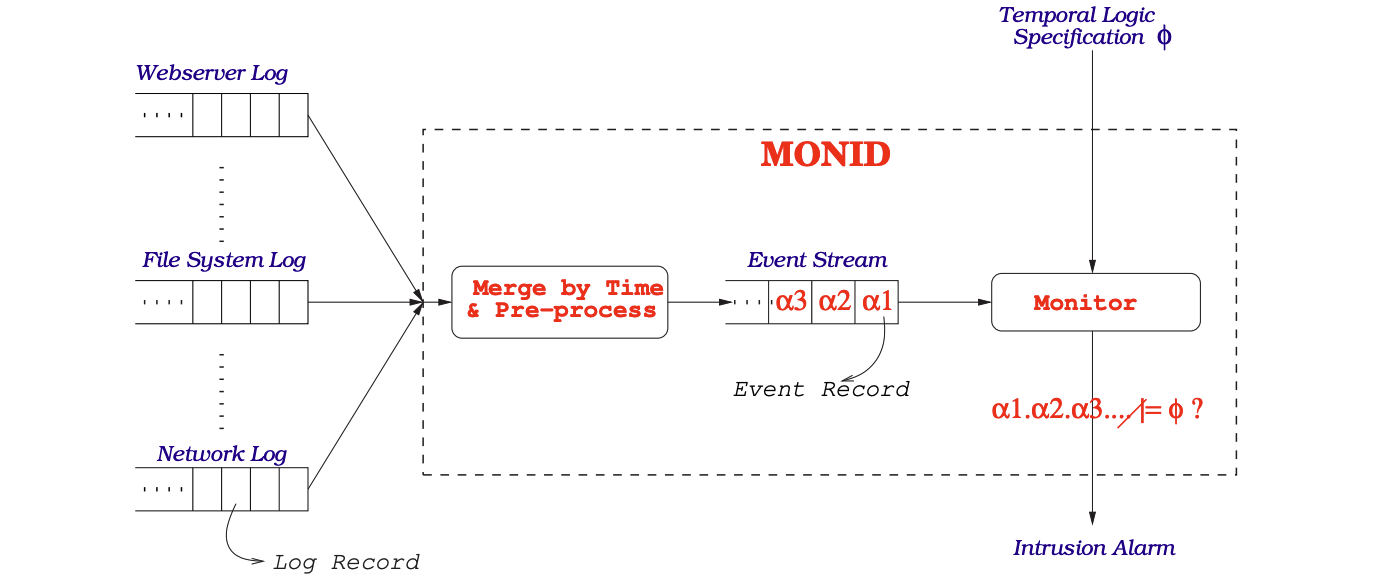
\includegraphics[width=\textwidth]{images/monid.png}
	\caption{MONID Architecture.}
	\label{monid}
\end{figure}

Some evaluations were also have been done in~\cite{naldurg2004temporal}, using the DARPA Intrusion Detection Evaluation dataset~\cite{mchugh2000testing}. The experiment was done using offline mode, against some of the attacks presented in Section~\ref{attacks}. More specifically, against the smurf, port-sweep and password-guessing attacks; the experiments detected 5 password-guess attack and 2 port-sweep attack in the logs and the performance overheads for monitoring the Port-Sweep and Password-Attacks are reported in Figure~\ref{graph1} and~\ref{graph2}, respectively. The X-axis in both graphs shows the number of events we are monitoring, as they are obtained from our logs. Each data point is the average overhead calculated for intervals of 10 and 1000 events respectively. The Y-axis plots the ratio between the time spent by the monitor vs. the time between the generation of the events in the actual log. As long as this ratio is less than 1, our monitoring is feasible. The results, show that the average overhead, is around $0.009$ for Port-Sweep attacks and $0.016$ for Password-Guessing attacks.
Although the used hardware is now outdated and obsolete, the overhead was rather modest, thus this method should still be theoretically helpful today.

\begin{figure}[!htb]
    \begin{center}
        \begin{minipage}{0.45\textwidth}
            \centering
            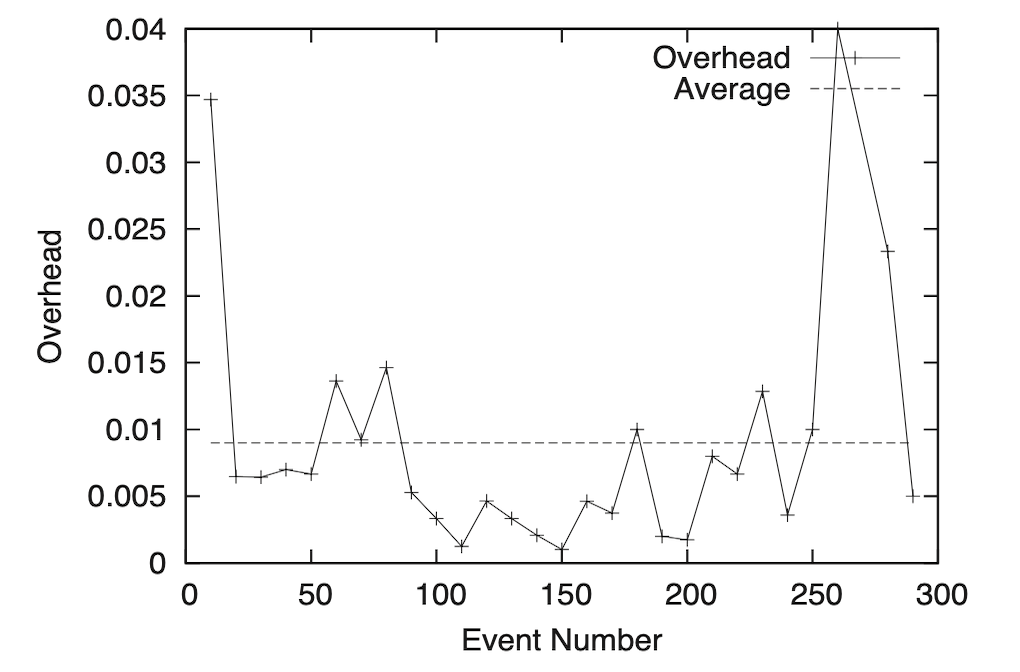
\includegraphics[width=1.1\linewidth]{images/graph 1.png}
            \caption{Performances overhead of Port-Sweep attacks.}\label{graph1}
        \end{minipage}
        \hfill
        \begin{minipage}{0.45\textwidth}
            \centering
            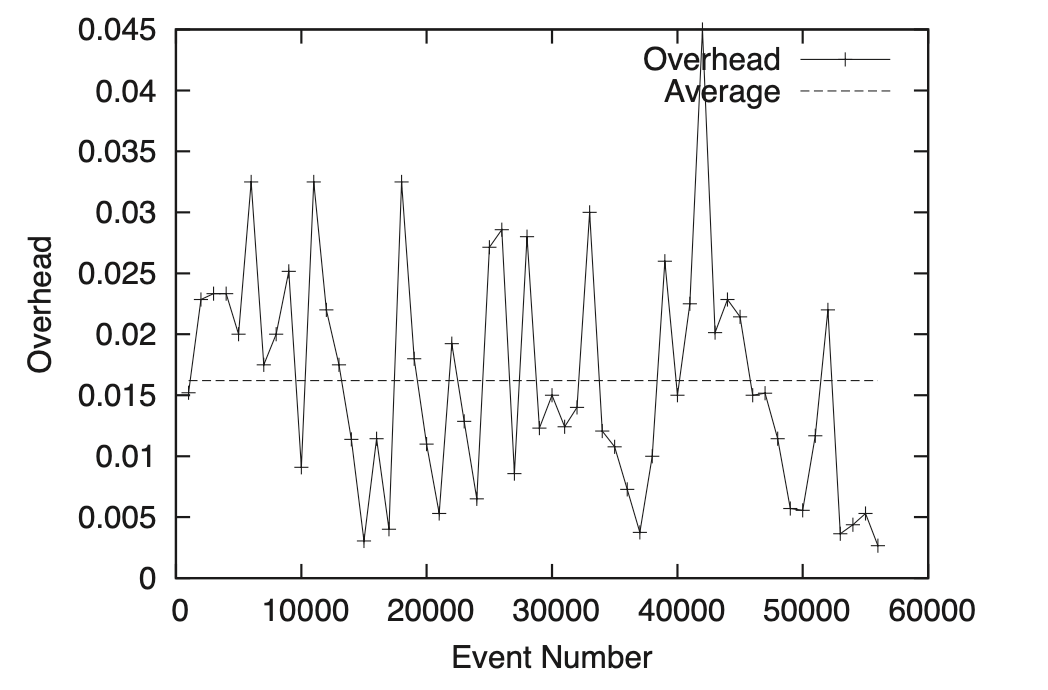
\includegraphics[width=1.1\linewidth]{images/graph 2.png}
            \caption{Performances overhead of Password-Guessing attacks.}\label{graph2}
        \end{minipage}
    \end{center}
\end{figure}


\section{Example of attacks}\label{attacks}
We give some examples of how EAGLE can be utilized to build formulas that correlate to desired execution trace characteristics of a system under observation in this section. In this context, a trace $\sigma$ that violates this specification is referred to as an intrusion or an attack; to explain how the framework may be used, we use examples from actual attacks illustrated in~\cite{naldurg2004temporal}. These illustrations demonstrate the expressive power of EAGLE formalism as well as its numerous features. In all the following examples, the rule Always is the one defined in Section~\ref{sec:ltl}.

\textbf{Smurf attacks.}
A smurf attack~\cite{zargar2009identification} is a type of Distributed Denial of Service (DDoS) attack that targets computer networks; in this scenario, the attacker sends a large volume of Internet Control Message Protocol (ICMP) echo request packets (commonly known as "ping" packets) to a network's broadcast address. This broadcast address is the address that reaches all devices on the targeted network. The attacker spoofs the source IP address of these ICMP packets to make it appear as if they are originating from the victim's IP address and since the broadcast address sends the request to all devices on the network, all devices will respond with ICMP echo replies to the victim's IP address. This results in a flood of traffic overwhelming the victim's network and causing it to become unreachable or severely degraded in performance. To detect this kind of attacks, we need to work on network logs; we will use a network tool called \textit{tcpdump}. The monitored formula that describes the absence of the attack is the following:
\begin{align*}
    & \underline{\text{max}}\ \mathtt{SmurfAttack()} = (type = \text{"ICMP"})\land isBroadcast(ip) \\
    & \underline{\text{mon}}\ \mathtt{SmurfSafety} =\ \mathtt{Always}(\neg\ \mathtt{SmurfAttack()}) 
\end{align*}
as we can see, the \textit{type} field of a record schema describes the type of network packet, while the \textit{ip} field is the destination of the packet. The $\mathtt{SmurfAttack}$ rule determines whether the packet is a ping packet and whether the source's IP address is a broadcast ip, i.e. all the host bits are set to 1. Thus, \textit{"Always there is no attack"} can be used to describe how the system behaves well in response to this attack.

\textbf{Cookie-stealing attacks.}
A cookie is a technique for tracking sessions that a web application server sends to a web client and uses to keep track of client-specific session data. These cookies that serve as authentication tokens are automatically included in requests by clients and in this scenario we assume that a session is exclusively identified by the client's IP address. When a malicious user uses an old cookie provided to a different IP address to take over a session, it is considered an attack.In order to monitor this attack we need to look at a web-server (application-level) log that contains a record of all sessions that the server participates in, along with session-specific state information.
According to the formula below, a specific cookie must always be utilized by the same IP address.

\begin{align*}
    & \underline{\text{min}}\ \mathtt{Hijack}(\underline{\text{string}}\ c,\underline{\text{string}}\ i) = ((name=c)\land\neg(ip=i))\lor\odot\ \mathtt{Hijack}(c,i) \\
    & \underline{\text{mon}}\ \mathtt{CookieSafe} =\ \mathtt{Always}(\neg\mathtt{Hijack}(name,ip)) 
\end{align*}
A trace that violates this formula therefore encodes a cookie-stealing attack. The rule $\mathtt{Hijack}$ checks wheter it occurs a situation in which we have the same coookie $c$ associated with two different ip $i$; if it's true then it means that a cookie has been stolen and reused by an attacker. With $\mathtt{CookieSafe}$ we want to check that it never occurs a situation just as the one described.

\textbf{Multi-domain Buffer Overflows attacks.}
According to~\cite{piromsopa2006buffer}, a buffer-overflow attack is an attack that (possibly implicitly) uses memory-manipulating operations to overflow a buffer which results in the modification of an address to point to malicious or unexpected code. In this case, we will integrate data from various log sources; to be more exact, we will examine both network and web server access logs to determine when a server buffer overflow attack has been performed. We search through network packets for binary data; then web server's access logs are examined to see if a corresponding event, in which the web server correctly terminates the connection after receiving some binary data, can be located. If no matching log record is discovered within a predetermined timeout, it means that the buffer overflow attack was successful. The following formulas captures this scenario:
\begin{align*}
    & \underline{\text{min}}\ \mathtt{EventuallyClosed}(\underline{\text{long}}\ t,\underline{\text{long}}\ d,\underline{\text{string}}\ i1,\underline{\text{string}}\ i2) = (time-t<d)\\
    & \quad\quad\land ((ip1=i1\land ip2=i2\land log=web\land type=closed)\lor \bigcirc\mathtt{EventuallyClosed}(t,d,i1,i2) ) \\
    & \underline{\text{mon}}\ \mathtt{BufferSafe} =\ \mathtt{Always}((log=network\land type=binary) \\
    & \quad\quad\rightarrow\mathtt{EventuallyClosed}(time,100,ip1,ip2))
\end{align*}
In each record we have the $log$ field which indicates the source of the log, the $time$ represents the istant in which the event occurs, $ip1$ represents the source address, $ip2$ represents the destination IP address and finally the $type$ field can be $binary, closed,\ldots$ We assume that a connection is identified by the tuple $(ip1,ip2)$. In order, the $\mathtt{EventuallyClosed}$ rule states that the connection between IP addresses $i1$ and $i2$ must end eventually within time $d$; finally, the monitor rule $\mathtt{BufferSafe}$ states that it is always the case that if there is an event of $binary$ access in the network log then eventually within time $100$ there must be a matching event in the webserver log that denotes the closing of the connection. 

\textbf{Password guessing attacks.}
Assuming the system accepts telnet connections to remote login; it won't take long until the password is compromised if an attacker is permitted to guess any amount of passwords for a specific user name. If a user guesses an incorrect password more than three times in a short amount of time, most systems end the telnet session. To prevent an attacker from succeeding by starting numerous temporary sessions, some systems cap the total number of unsuccessful login attempts over a longer time frame; in this case we need to have access to the host's audit logs. The formulas that capture this scenario are the following:
\begin{align*}
    & \underline{\text{max}}\ \mathtt{Failure}() = (type=login)\land \neg success\\
    & \underline{\text{max}}\ \mathtt{Guess}(\underline{\text{string}}\ i) = (ip=i)\land \mathtt{Failure}()\\
    & \underline{\text{max}}\ \mathtt{Counter}(\underline{\text{long}}\ t, \underline{\text{long}}\ d, \underline{\text{int}}\ c,\underline{\text{string}}\ i,\underline{\text{int}}\ C) = (time-t<d)\\
    & \quad\quad\rightarrow((\mathtt{Guess}(i)\rightarrow(c\leq C\land \bigcirc\mathtt{Counter}(t,d,c+1,i,C)))  \\
    & \quad\quad\land(\neg \mathtt{Guess}(i)\rightarrow\mathtt{Counter}(t,d,c,i,C))) \\
    & \underline{\text{mon}}\ \mathtt{PassGuessSafe} =\ \mathtt{Always}(\mathtt{Failure}()\rightarrow\mathtt{Counter}(time,300,1,ip,3)) 
\end{align*}
as we can see, the rules here are numerous. In $\mathtt{Counter}$, the arguments $t, d, c, i, C$ represent the rule invocation time, the timeout period, the current number of unsuccessful-guesses count, the source IP address doing the guess, and the threshold count. When the number of guesses from the IP address $i$ exceeds the threshold count $C$ within the timeout period $d$, an attack has taken place. The parameterized rule $\mathtt{Counter}$ starts with the initial count $c$ set to 1 whenever there is a $\mathtt{Failure}$ during login. The number of guesses is increased by one for each instance of an event signifying a failed login attempt from the same IP address within the timeout period $d$. The rule $\mathtt{Counter}$ also determines whether the local counter $c$ surpasses the threshold $C$ within time d, and if it does, the entire rule become false, indicating an attack. Finally, with the rule $\mathtt{PassGuessSafe}$ we assure that whenever there is a failed login from a specific IP address, we make sure that within time $300$ seconds the number of login-failures from the same IP address must be less than or equal to $3$.

\textbf{Port Scanning attacks.}
According to~\cite{kanlayasiri2000rule}, Port scanning attack is a method for discovering exploitable communication channels that has been used for a long time. The key idea is to probe the network ports and then keep the information about them that are useful for an attack.
Hackers frequently employ a port scan approach to find gaps or weak spots in a network. Attackers can use a port scan attack to identify open ports and determine if they are accepting or rejecting data; additionally, it can show whether a company uses firewalls or other active security measures. 
Assuming that our server has multiple network inferfaces, thus multiple IP addresses; the victim machine can presume that port scans are malicious when the counter of reached ports overcomes a specific threshold in a short amount of time. The formulas are the following:
\begin{align*}
    & \underline{\text{max}}\ \mathtt{NewPort}(\underline{\text{string}}\ i1,\underline{\text{string}}\ i2,\underline{\text{Set}}\ S) = (i1=ip1)\land(i2=ip2)\land (port \notin S)\\
    & \underline{\text{max}}\ \mathtt{Counter}(\underline{\text{long}}\ t, \underline{\text{long}}\ d, \underline{\text{int}}\ c,\underline{\text{string}}\ i1,\underline{\text{string}}\ i2,\underline{\text{Set}}\ S,\underline{\text{int}}\ C) = (time-t<d)\\
    & \quad\quad\rightarrow((\mathtt{NewPort}(i1,i2,S)\rightarrow(c\leq C\land \bigcirc\mathtt{Counter}(t,d,c+1,i1,i2,S\cup\{port\},C)))  \\
    & \quad\quad\land(\neg \mathtt{NewPort}(i1,i2,S)\rightarrow\mathtt{Counter}(t,d,c,i1,i2,S,C))) \\
    & \underline{\text{mon}}\ \mathtt{PortScanSafe} =\ \mathtt{Always}(\mathtt{Counter}(time,100,1,ip1,ip2,\{port\},10)) 
\end{align*}
in this case we have two IPs; $ip1$ is the source IP, while $ip2$ is the destination one. The parameterized $\mathtt{Counter}$ rule states that the number of port scans between a source and destination IP  address pair $(i1,i2)$ recorded do not surpass a threshold $C$ within time $d$. The rule $\mathtt{NewPort}$ checks if the port number,
involved in any communication between the IP addresses $i1$ and $i2$, exists in the set $S$ of all port numbers (involved in all communications between $i1$ and $i2$) within the timeout period $d$.

\section{Conclusions}
In conclusion, we have introduced a new temporal logic named EAGLE, which serves as the foundation for the MONID framework, which is a useful tool for system intrusion detection.
MONID continuously monitor these attack specifications during system execution and when the observed execution contradicts the monitored formula, we detect an intrusion. We have showcased this by creating formulas to identify several common attacks and testing our monitoring algorithm on large event logs provided by DARPA. These examples can serve as templates for specifying many other types of attacks. The obtained results were excellent, both in terms of detected attacks and system overhead.

\printbibliography

\end{document}